\documentclass[11pt]{article}
\usepackage{amsmath,amssymb,amsthm}
\usepackage{graphicx}
\usepackage{url}
\usepackage{hyperref}
\usepackage{color}
\usepackage{algorithm,algorithmic}
\usepackage[T1]{fontenc}

\hypersetup{
    colorlinks=true,
    linkcolor=blue,
    filecolor=magenta,      
    urlcolor=cyan,
}


\newcommand{\INPUT}{\item[{\bf Input:}]}
\newcommand{\OUTPUT}{\item[{\bf Output:}]}
\newcommand{\RR}{{\mathbb R}}
\newcommand{\myvec}[1]{\mathbf{#1}}
\newcommand{\ignore}[1]{}%


\DeclareMathOperator*{\E}{\mathbb{E}}
\let\Pr\relax
\DeclareMathOperator*{\Pr}{\mathbb{P}}
%\DeclareMathOperator*{\myv}{\mathbf{#1}}
\newcommand{\mv}[1]{\mathbf{#1}}
\newcommand{\mynorm}[1]{\|{#1}\|}


\newcommand{\eps}{\varepsilon}
\newcommand{\inprod}[1]{\left\langle #1 \right\rangle}

\newcommand{\handout}[5]{
  \noindent
  \begin{center}
  \framebox{
    \vbox{
      %\hbox to 5.78in { {\bf AM 221: Advanced Optimization } \hfill #2 }
            \hbox to 6.38in { {\bf AM 221: Advanced Optimization } \hfill #2 }
      \vspace{4mm}
      %\hbox to 5.78in { {\Large \hfill #5  \hfill} }
            \hbox to 6.38in { {\Large \hfill #5  \hfill} }
      \vspace{2mm}
            \hbox to 6.38in { {\em #3 \hfill #4} }
      %\hbox to 5.78in { {\em #3 \hfill #4} }
    }
  }
  \end{center}
  \vspace*{4mm}
}

\newcommand{\lecture}[3]{\handout{#1}{#2}{#3}{Lecture #1}}
\newcommand{\homework}[3]{\handout{#1}{#2}{#3}{Problem Set #1}}
\newcommand{\sect}[3]{\handout{#1}{#2}{#3}{Section #1}}

\newtheorem{theorem}{Theorem}
\newtheorem{corollary}[theorem]{Corollary}
\newtheorem{lemma}[theorem]{Lemma}
\newtheorem{observation}[theorem]{Observation}
\newtheorem{proposition}[theorem]{Proposition}
\newtheorem{definition}[theorem]{Definition}
\newtheorem{claim}[theorem]{Claim}
\newtheorem{fact}[theorem]{Fact}
\newtheorem{assumption}[theorem]{Assumption}

\newtheorem*{theorem*}{Theorem}
\newtheorem*{corollary*}{Corollary}
\newtheorem*{conjecture*}{Conjecture}
\newtheorem*{lemma*}{Lemma}
\newtheorem*{thm*}{Theorem}
\newtheorem*{prop*}{Proposition}
\newtheorem*{obs*}{Observation}
\newtheorem*{definition*}{Definition}
\theoremstyle{remark}
\newtheorem{remark}[theorem]{Remark}
\newtheorem*{example}{Example}
\newtheorem*{rem*}{Remark}
\newtheorem*{rec*}{Recommendation}


% 1-inch margins, from fullpage.sty by H.Partl, Version 2, Dec. 15, 1988.
\topmargin 0pt
\advance \topmargin by -\headheight
\advance \topmargin by -\headsep
\textheight 8.9in
\oddsidemargin 0pt
\evensidemargin \oddsidemargin
\marginparwidth 0.5in
\textwidth 6.5in

\parindent 0in
\parskip 1.5ex

%Basics
\newcommand{\new}[1]{{\em #1\/}}		% New term (set in italics).

\newcommand{\boxdef}[1]
{
\fbox{
\begin{minipage}{42em}
\begin{definition*}
{#1}
\end{definition*}
\end{minipage}
}
}

\newcommand{\boxthm}[1]
{
\fbox{
\begin{minipage}{42em}
\begin{theorem*}
{#1}
\end{theorem*}
\end{minipage}
}
}

\newcommand{\boxfact}[1]
{
\fbox{
\begin{minipage}{42em}
%\begin{theorem*}
\emph{{#1}
%\end{theorem*}
}
\end{minipage}
}
}




%Probability
\newcommand{\prob}[2][]{\text{\bf P}\ifthenelse{\not\equal{}{#1}}{_{#1}}{}\!\left(#2\right)}
\newcommand{\expect}[2][]{\text{\bf E}\ifthenelse{\not\equal{}{#1}}{_{#1}}{}\!\left[#2\right]}
\newcommand{\var}[2][]{\text{\bf Var}\ifthenelse{\not\equal{}{#1}}{_{#1}}{}\!\left[#2\right]}

%Sets
\newcommand{\set}[1]{\{#1\}}			% Set (as in \set{1,2,3})
\newcommand{\given}{\, : \,}
\newcommand{\setof}[2]{\{{#1} \given {#2}\}}	% Set (as in \setof{x}{x > 0})
\newcommand{\compl}[1]{\overline{#1}}		% Complement of ...            
\newcommand{\zeros}{{\mathbf 0}}
\newcommand{\ones}{{\mathbf 1}}
\newcommand{\union}{{\bigcup}}
\newcommand{\inters}{{\bigcap}}

%Other Math
\newcommand{\floor}[1]{{\lfloor {#1} \rfloor}}
\newcommand{\bigfloor}[1]{{\left\lfloor {#1} \right\rfloor}}
\DeclareMathOperator{\argmax}{argmax}
\DeclareMathOperator{\argmin}{argmin}

\newcommand{\PRIMAL}{{\textsc{Primal}}}
\newcommand{\DUAL}{{\textsc{Dual}}}



%Numbers
\newcommand{\C}{\mathbb{C}}	                % Complex numbers.
\newcommand{\N}{\mathbb{N}}                     % Positive integers.
\newcommand{\Q}{\mathbb{Q}}                     % Rationals.
\newcommand{\R}{\mathbb{R}}                     % Reals.
\newcommand{\Z}{\mathbb{Z}}                     % Integers.
\newcommand{\M}{\mathcal{M}}                     % Matroids.
\newcommand{\I}{\mathcal{I}}                     % Independent Sets.

%Headings
\newcommand{\parta}{\textbf{(a)}}
\newcommand{\partb}{\textbf{(b)}}
\newcommand{\partc}{\textbf{(c)}}
\newcommand{\partd}{\textbf{(d)}}
\newcommand{\parte}{\textbf{(e)}}


\newcommand{\bt}{\boldsymbol{\theta}}
\newcommand{\cl}[1]{\text{\textbf{#1}}}
\newcommand{\eqdef}{\mathbin{\stackrel{\rm def}{=}}}
\newcommand{\bx}{\mathbf{x}}
\newcommand{\bq}{\mathbf{q}}
\newcommand{\by}{\mathbf{y}}
\newcommand{\bb}{\mathbf{b}}
\newcommand{\bu}{\mathbf{u}}
\newcommand{\bd}{\mathbf{d}}
\newcommand{\ba}{\mathbf{a}}
\newcommand{\bc}{\mathbf{c}}
\newcommand{\bl}{\mathbf{l}}
\newcommand{\bp}{\mathbf{p}}
\newcommand{\bw}{\mathbf{w}}
\newcommand{\bz}{\mathbf{z}}


\begin{document}
\homework{7 (updated)  --- {\color{red} Due Wednesday, Mar. 21st at 23:59}}{Spring
  2018}{Kojin Oshiba}

%\renewcommand{\abstractname}{}
\paragraph{Instructions:}

\begin{itemize}
\item 
All your solutions should be prepared in \LaTeX \ and the
PDF and .tex should be submitted to Canvas. 
	Please submit all your files as ONE archive of filetype zip, 
        tgz, or tar.gz.
\item
Name the file
  {[your-first-name]}\_{[your-last-name]}.{[filetype]}.
  For example, I would call my submission
  rasmus\_kyng.zip. 
\item 
INCLUDE your name in the submisson pdf and any files with code.
\item 
{\color{red}
If the TFs cannot easily deduce your identity from your files alone, they may
decide not to grade your submission.
}
\item 
For each question, a
well-written and
correct answer will be selected a sample solution for the entire class to
enjoy.  If you prefer that we do not use your solutions, please indicate this
clearly on the first page of your assignment. 
\end{itemize}


\paragraph{1. Entropy maximization.}

In this problem, we will consider the \emph{entropy maximization problem}. Let
us consider a probability distribution $\bx\in\R^n$ over a finite set of size
$n$. We have $\bx\geq 0$ and $\sum_{i=1}^n x_i = 1$. The entropy of $\bx$ is
defined by:
\begin{displaymath}
    H(\bx) = \sum_{i=1}^n x_i\log \frac{1}{x_i}
\end{displaymath}
We are interested in maximizing entropy, or equivalently, solving the following
problem:
\begin{displaymath}
    \begin{aligned}
        \min_{\bx\in\R^n}&\; \sum_{i=1}^nx_i\log x_i\\
        \text{s.t} &\; \sum_{i=1}^n x_i = 1\\
                   &\; \bx\geq 0
    \end{aligned}
\end{displaymath}

\begin{itemize}
    \item[a.] Prove Jensen's inequality: let $f:\R^n\to\R$ be a strictly convex
        function, let $\bx_1,\dots\bx_m$ by $m$ vectors in $\R^n$, and let
        $\lambda_1,\dots,\lambda_m$ be such that $\sum_{i=1}^m\lambda_i=1$ and
        $\lambda_i\geq 0,\;1\leq i\leq m$, then:
        \begin{displaymath}
            f\left(\sum_{i=1}^m\lambda_i\bx_i\right)
            \leq \sum_{i=1}^m\lambda_if(\bx_i)
        \end{displaymath}
        and prove that the inequality is an equality if and only if
        $\bx_1=\bx_2=\dots=\bx_m$.
    \item[b.] Using Jensen's inequality, what is the optimal solution to the
        entropy maximization problem above? Specify both the distribution $\bx$
        of maximum entropy and the value of its entropy.
    \item[c.] We now add the constraint $A\bx\leq b$ to the entropy
        maximization problem, where $A\in\R^{m\times n}$ and $\bb\in\R^m$. The
        problem now becomes:
\begin{displaymath}
    \begin{aligned}
        \min_{\bx\in\R^n}&\; \sum_{i=1}^nx_i\log x_i\\
        \text{s.t} &\; \sum_{i=1}^n x_i = 1\\
                   &\; \bx\geq 0\\
                   &\; A\bx\leq \bb
    \end{aligned}
\end{displaymath}
Show that the dual of this problem can be written in the following form:
\begin{displaymath}
    \begin{aligned}
        \max_{\nu\in\R^m}&\; -\bb^\intercal \nu
        -\log\left(\sum_{i=1}^ne^{-\ba_i^\intercal \nu}\right)\\
        \text{s.t} &\; \nu\geq 0\\
    \end{aligned}
\end{displaymath}
where $\ba_i$ is the $i$th column of $A$. Assuming that strong duality holds
for this problem, re-derive the result of part b. by considering a pair of
primal/dual optimal solutions.
\end{itemize}

\color{blue}
\begin{itemize}
\item[a.]
We show this by induction. When $m=2$, because $f$ is convex,
$$f(\lambda_1\bx_1+\lambda_2\bx_2) \leq \lambda_1 f(\bx_1)+\lambda_2f(\bx_2)$$
Suppose $f\left(\sum_{i=1}^m\lambda_i\bx_i\right)
            \leq \sum_{i=1}^m\lambda_if(\bx_i)$ for $m=k$. Then, for $m=k+1$,

\begin{align*}
f\left(\sum_{i=1}^m\lambda_i\bx_i\right) &= f(\lambda_{k+1}\bx_{k+1} + \sum_{i=1}^k \lambda_i\bx_i) &\\
&= f(\lambda_{k+1}\bx_{k+1} + (1-\lambda_{k+1})\sum_{i=1}^k \frac{\lambda_i}{1-\lambda_{k+1}}\bx_i &\\
&\leq  \lambda_{k+1} f(\bx_{k+1}) + (1-\lambda_{k+1})f(\sum_{i=1}^k \frac{1}{1-\lambda_{k+1}}\bx_i) &\\
\end{align*}

Since $\sum_{i=1}^{k+1}\lambda_i=1, 1-\lambda_{k+1} = \sum_{i=1}^k \lambda_i$. Hence, $\sum_{i=1}^k \frac{1}{1-\lambda_{k+1}}= 1$. \\
So, $f(\sum_{i=1}^k \frac{1}{1-\lambda_{k+1}}\bx_i) \leq \frac{1}{1-\lambda_{k+1}} \sum_{i=1}^k \lambda_i f(\bx_i)$.
Therefore,
\begin{align*}
f(\sum_{i=1}^m\lambda_i\bx_i) &\leq  \lambda_{k+1} f(\bx_{k+1}) + \sum_{i=1}^k \lambda_i f(\bx_i) &\\
&= \sum_{i=1}^{k+1} \lambda_i f(\bx_i)
\end{align*}

When $\bx_1=...=\bx_m$, \\ 
$$f\left(\sum_{i=1}^m\lambda_i\bx_i\right)=f(\bx_i),\sum_{i=1}^m\lambda_if(\bx_i)=f(\bx_i)$$

The converse is true by induction analogous to the above proof: using the fact that in the base case, $f(\lambda_1\bx_1+\lambda_2\bx_2)=\lambda_1f(\bx_1)+\lambda_2f(\bx_2)$ implies $\bx_1=\bx_2$ because $f$ is strictly convex.

\item[b.]
First, 
$$min \sum_{i=1}^nx_i logx_i=min \ n\sum_{i=1}^n \frac{1}{n}x_i logx_i$$
Since $f(x)=xlogx$ is convex for $0 \leq x \leq 1$,

$$\sum_{i=1}^n \frac{1}{n}x_i logx_i \geq f(\sum_{i=1}^n \frac{1}{n}x_i) = (\sum_{i=1}^n \frac{1}{n}x_i)log(\sum_{i=1}^n \frac{1}{n}x_i)$$
When $x_1=...=x_n=x$,
$$-n(\sum_{i=1}^n \frac{1}{n}x_i)log(\sum_{i=1}^n \frac{1}{n}x_i) = -nxlogx=logn$$

\item[c.]
The langrangian is
\begin{align*}
L(\bx,\lambda,\nu)&=\sum_{i=1}^n x_ilogx_i + \nu^\intercal (A\bx-\textbf{b}) + \lambda(1^\intercal \bx -1)&\\
&=-b^\intercal -\lambda + \sum_{i=1}^n x_i (logx_i+a_i^\intercal \nu + \lambda) 
\end{align*}

$$\frac{\partial}{\partial x_i} L(\bx,\lambda,\nu)=\frac{\partial}{\partial x_i} x_i (logx_i+a^\intercal_i \nu+\lambda)$$
To minimize $L(x,\lambda,\nu)$, set this to $0$, which results in
$$x_i^*=exp(-a_i^\intercal \nu - \lambda - 1)$$

Hence, $$inf_{\bx} L(\bx,\nu,\lambda)=L(\bx^*,\nu,\lambda)=-b^\intercal \nu -\lambda - \sum_{i=1}^n exp(-a_i^\intercal \nu - \lambda - 1)$$

Now, let's find the optimal $\lambda$.
$$\frac{\partial}{\partial \lambda}  L(\bx^*,\nu,\lambda) = -1 + \sum_{i=1}^n exp(-a_i^\intercal \nu - \lambda - 1)$$

Setting this to $0$ and solving for $\lambda$ results in

$$\lambda* = log( \sum_{i=1}^n exp(-a_i^\intercal \nu - 1)$$

Hence,
\begin{align*}
L(\bx^*,\nu,\lambda*) &=-b^\intercal \nu -\lambda* + \sum_{i=1}^n x_i (logx_i+a_i^\intercal \nu + \lambda) &\\
&= -b^\intercal \nu -\lambda* + 1 &\\
&= -b^\intercal \nu + log(\sum_{i=1}^n x_i  exp(-a_i^\intercal \nu))
\end{align*}

\end{itemize}
\color{black}

\paragraph{2. Minimum volume ellipsoid.}

An ellipsoid in $\R^d$ is the image of the unit ball by a linear invertible map, i.e a set $\mathcal{E}$ defined by:
\begin{displaymath}
    \mathcal{E} = \{A\bx: \bx\in\R^d,\;\|\bx\|_2\leq 1\}
\end{displaymath}
for some invertible linear map $A:\R^d\mapsto\R^d$. In this case, we define the volume of the ellipsoid to be $|\det A|$. An equivalent parametrization of the ellipsoid is:
\begin{displaymath}
    \mathcal{E} = \{\by\in\R^d: \by^\intercal W \by\leq 1\}
\end{displaymath}
with $W = (A^{-1})^\intercal A^{-1}$. Note that $W$ is symmetric positive definite and that under this parametrization, the volume of the ellipsoid is $(\det W)^{-1/2}$.

Let us denote by $\mathbf{S}_d^{++}$ the set of symmetric positive definite
matrices of size $d\times d$. Given $n$ points $\bx_1,\ldots, \bx_n$ in $\R^d$,
the \emph{minimum volume ellipsoid} problem consists in finding the ellipsoid
of minimum volume containing all points $\bx_1,\ldots, \bx_n$, that is:
\begin{displaymath}
    \begin{split}
        \min_{W\in\mathbf{S}_d^{++}}&\; (\det W)^{-1/2}\\
        \mathrm{s.t.}&\; \bx_i^\intercal W\bx_i\leq 1,\; 1\leq i\leq n
    \end{split}
\end{displaymath}

\begin{itemize}
    \item[a.] Show that $\mathbf{S}_d^{++}$ is convex.
    \item[b.] Let us define $d: \mathbf{S}_d^{++}\rightarrow\R$ by $d(W) = (\det W)^{-1/2}$. Is $d$ convex over $\mathbf{S}_d^{++}$?
\end{itemize}
Using the fact that $\log$ is increasing over $\R^+\setminus\{0\}$, we consider
the following problem which is equivalent to the minimum volume ellipsoid
problem:
\begin{equation}\label{P}
    \begin{split}
        \min_{W\in\mathbf{S}_d^{++}}&\; \log\det (W^{-1})\\
        \mathrm{s.t.}&\; \bx_i^\intercal W\bx_i\leq 1,\; 1\leq i\leq n
    \end{split}
\end{equation}
\begin{itemize}
    \item[c.] Show that the function $f$ defined by $f(W) = \log\det(W^{-1})$
        is convex and differentiable over $S_d^{++}$ and that $\nabla f(W)
        = -W^{-1}$.
    \item[d.] Show that the dual of problem \eqref{P} is:
        \begin{displaymath}
            \begin{split}
            \max_{\lambda\in\R^n}&\;
            \log\det\Bigg(\sum_{i=1}^n\lambda_i\bx_i\bx_i^\intercal\Bigg)
            - \sum_{i=1}^n \lambda_i + d\\
            \mathrm{s.t.}&\; \lambda\geq 0,\; \sum_{i=1}^n \lambda_i
            \bx_i\bx_i^\intercal\in\mathbf{S}_d^{++}
        \end{split}
        \end{displaymath}
    \item[e.] Show that the dual can be further simplified to:
        \begin{equation}\label{d2}
            \begin{split}
            \max_{\lambda\in\R^n}&\;
            \log\det\Bigg(\sum_{i=1}^n\lambda_i\bx_i\bx_i^\intercal\Bigg)
            +d\log d\\
            \mathrm{s.t.}&\; \lambda\geq 0,\; \sum_{i=1}^n \lambda_i
            \bx_i\bx_i^\intercal\in\mathbf{S}_d^{++}, \sum_{i=1}^n \lambda_i = 1
        \end{split}
        \end{equation}
\end{itemize}

\color{blue}
\begin{itemize}
\item[a.]
For $A_1,A_2\in S_d^{++}$, 
$$(\lambda A_1+(1-\lambda)A_2)^\intercal = \lambda A_1^\intercal + (1-\lambda)A_2^\intercal = \lambda A_1+ (1-\lambda)A_2 $$
Moreover,
$$\bx^\intercal (\lambda A_1+(1-\lambda)A_2) \bx = \lambda \bx^\intercal A_1 \bx + (1-\lambda) \bx^\intercal A_2 \bx > 0$$
Hence,
$$\lambda A_1+ (1-\lambda)A_2 \in S_d^{++}$$
Thus, $S_d^{++}$ is convex.

\item[b.]
$$(detW)^{-\frac{1}{2}}=exp(-\frac{1}{2}logdet(W))$$
Since$logdet$ is concave from (c), $-logdet$ is convex. Moreover, we have that $exp$ is convex and monotonically increasing. Since $f\circ g$ is convex if $f$ is convex and $g$ is convex and monotonically increasing, we have that $(detW)^{-\frac{1}{2}}$ is convex.

\item[c.]
To show this, it suffices to show that $logdet(W)$ is concave. To show this, let $g(t)=f(W+tX)$ where $W,X \in S_d^{++}$. Since  $S_d^{++}$ is convex, $W+tX \in S_d^{++}$ as well. Now,
\begin{align*}
g(t) &= logdet(W+tX) &\\
&= logdet(W^{1/2}(I+tW^{-1/2}XW^{1/2})W^{1/2} &\\
&= \sum_{i=1}^n log(1+t\lambda_i)+logdet W
\end{align*}
where $\lambda_i$'s are eigen values of $W^{-1/2}XW^{1/2})W^{1/2}$. Hence, 
$$g''(t) = -\sum_{i=1}^n \frac{\lambda_i^2}{(1+t\lambda_i)^2} \leq 0$$

Hence, we have that $f$ is concave.

\item[d.]
$$L(W,\lambda)=logdet(W^{-1})+\sum_{i=1}^n \lambda_i(\bx_i^\intercal W \bx_i-1)$$
Hence, 
$$\frac{\partial L(W,\lambda)}{\partial W} = -W^{-1}+\sum_{i=1}^n \lambda_i \bx_i^\intercal \bx_i$$
Setting this to $0$ reuslts in
$$W^{*-1} = \sum_{i=1}^n \lambda_i \bx_i^\intercal \bx_i$$
So,
$$L(W^*,\lambda)=logdet(\sum_{i=1}^n \lambda_i \bx_i^\intercal \bx_i) + \sum_{i=1}^n \lambda_i  \bx_i^\intercal W \bx_i - \sum_{i=1}^n \lambda_i $$
Now,
\begin{align*}
tr(\sum_{i=1}^n \lambda_i  \bx_i^\intercal W \bx_i)&=\sum_{i=1}^n \lambda_i  tr(\bx_i^\intercal W \bx_i) &\\
&= \sum_{i=1}^n \lambda_i  tr(W \bx_i \bx_i^\intercal) &\\
&= tr(W \sum_{i=1}^n \lambda_i \bx_i \bx_i^\intercal) &\\
&= tr(I) &\\
&= d
\end{align*}
Hence,
$$L(W^*,\lambda)=logdet(\sum_{i=1}^n \lambda_i \bx_i^\intercal \bx_i) + d - \sum_{i=1}^n \lambda_i$$
which is the objective we would like to have.
Finally the constraint $\sum_{i=1}^n \lambda_i
            \bx_i\bx_i^\intercal\in\mathbf{S}_d^{++}$ comes from the fact that we want $W^{-1}$ to be positive definite.
            
\item[e.]
Let $\sum_{i=1}^n \lambda'_i=1, \lambda' \geq 0$. This will correspond to the $\lambda_i$'s in e, as we will show. Let $S=\sum_{i=1}^n \lambda_i=$ be the sum of $\lambda_i$'s in d. Let $\lambda_i=\lambda_i' S$. Then, we have that
$$logdet(\sum_{i=1}^n\lambda\bx_i\bx_i^\intercal)-\sum_{i=1}^n\lambda_i+d = logdet(S \sum_{i=1}^n \lambda'_i \bx_i\bx_i^\intercal)-S+d$$
Maximizing this with respect to S by taking the derivative and setting this to $0$, we have $S=d$. Hence, the objective now becomes
$$ logdet(\sum_{i=1}^n \lambda'_i \bx_i\bx_i^\intercal)-dlogd$$ with the constraint that $\sum_{i=1}^n \lambda'_i=1$
We can rewrite $\lambda'_i$ as $\lambda_i$ to get the notations as specified in the problem.

\end{itemize}
\color{black}

\paragraph{3. Support vector machines.}

In this problem, we will use a dataset on forged
banknotes. We will use support
vector machines to construct a classifier that tries to predict if
notes are forged.  The dataset is available at
\url{http://rasmuskyng.com/am221_spring18/psets/hw7/banknotes.data}.
In each line, the first four columns contain measurements from a banknote (real numbers) and the last column
is a binary (0 or 1) variable indicating if the banknote was forged. Denoting
by $\bx^i\in\R^4$ the measurements from banknote $i$, the goal is to construct
a classifier which takes $\bx^i$ as input and predicts the last column
$y^i\in\{0, 1\}$.

First, convert the labels to $\hat{y}^i\in\{-1, 1\}$, i.e. $\hat{y}^i
= 2y^i - 1$.
%
As seen in class, finding a separating hyperplane now amounts to
finding $\bw\in\R^d$ and $b \in \R$ such that
$\hat{y}^i (\bw^\intercal\bx_i +b)\geq 1$ , for $1\leq i\leq n$, where $\bx_1,\dots\bx_n$ are
the (modified) data points.

As seen in class, the optimization problem for support vector machines now
takes the following form:
\begin{displaymath}
    \begin{aligned}
        \min_{\bw\in\R^d, b \in \R}&\; \frac{1}{2}\|\bw\|^2\\
        \text{s.t} &\; \hat{y}^i (\bw^\intercal\bx_i +b)\geq 1,\;1\leq i\leq n
    \end{aligned}
\end{displaymath}

In cases where the dataset is not linearly separable, it is not possible to
find $\bw$ satisfying the constraints of the above problem. In particular, we
might have $\hat{y}^i (\bw^\intercal\bx_i +b) < 1$ for some $i$. If this is the
case, there exists $\xi_i\geq 0$ such that $\hat{y}^i
(\bw^\intercal\bx_i +b) + \xi_i \geq 1$.
The number $\xi_i$ quantifies the ``misclassification'' of data point $i$.
Since we want to discourage these misclassifications, we incorporate them into
the objective function and consider the following optimizing problem instead:
\begin{equation}
    \label{eq:bar}
    \begin{aligned}
        \min_{\bw\in\R^d,\, b \in  \R, \xi\in\R^n}&\; \frac{1}{2}\|\bw\|^2
        + \lambda\sum_{i=1}^n\xi_i\\
        \text{s.t} &\; \hat{y}^i(\bw^\intercal\bx_i +b) + \xi_i \geq 1 ,\;1\leq i\leq n\\
                   &\; \xi_i\geq 0,\;1\leq i\leq n
    \end{aligned}
\end{equation}
where $\lambda$ is a parameter that we can choose depending on how much we want
to penalize misclassified data points.

\begin{itemize}
    \item[a.] Reuse your implementation of the perceptron algorithm
      from HW2, Question 5d and run it
        on the banknote dataset. Which behavior do you observe? Can you explain
        why?
    \item[b.] Use a convex solver to solve the convex program \eqref{eq:bar}.
        Note that the objective function is quadratic, so you can use
        a function specific to quadratic problems. In CVXOPT, this is the
        \textsf{cvxopt.solvers.qp} function. Solve the problem for different
        values of $\lambda$ and plot the classification accuracy
        (fraction of the data points that were correctly classified)
        as a function of $\lambda$. How do you explain the shape of this plot?
    \item[c.] Show that the program \eqref{eq:bar} is equivalent to the
        following problem:
\begin{equation}
    \label{eq:bar2}
    \begin{aligned}
        \min_{\bw\in\R^d, b\in \R}&\; \frac{1}{2}\|\bw\|^2
        + \lambda\sum_{i=1}^n\max(0,1-\hat{y}^i (\bw^\intercal\bx_i +b))\\
    \end{aligned}
\end{equation}
\item[d.]\textbf{[Optional, for bonus credits]} The advantage of problem
    \eqref{eq:bar2} is that it is unconstrained. So we can use subgradient
    descent to solve it. Run the subgradient descent algorithm to solve Problem
    \eqref{eq:bar2} for the best value of $\lambda$ found in part b.
\item[e.]\textbf{[Optional, for bonus credits]} Note that \eqref{eq:bar2} also
    has a ``separable'' objective function as seen in Stochastic Gradient
    Descent (section 7). Implement the Stochastic Gradient descent algorithm
    and use it to solve \eqref{eq:bar2}. Compare the number of iterations
    required to reach the same accuracy with gradient descent (part d.) and
    stochastic gradient descent (part e.).
\end{itemize}

\color{blue}
\begin{itemize}
\item[a.]
The implementation is at `hw7.py`.
The perceptron doesn't hult, since the data is not linearly separable.

\item[b.]
I observe that the larger lambda is the higher the accuracy is. This makes sense because as lambda increases, we are penalizing the size of the slack variables more, meaning that we are being more strict to the points misclassified.

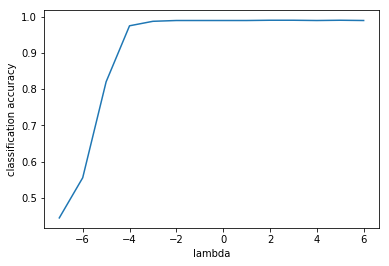
\includegraphics{hw7}

\item[c.]
\begin{align*}
& \xi_i \geq 0, \hat{y}^i(\bw^\intercal \bx_i + b)+\xi_i \geq 1 &\\
\Leftrightarrow & \xi_i \geq 0, \xi_i \geq 1 - \hat{y}^i(\bw^\intercal \bx_i + b)&\\
\Leftrightarrow & \xi_i \geq max(0, 1- \hat{y}^i(\bw^\intercal \bx_i + b))
\end{align*}

Hence, we can replace $\xi_i$ in the minimization problem with its lower bound.

\end{itemize}
\color{black}

\end{document}
